\subsubsection{Exotic Higgs Decays to $Z_D Z$, $Z_D Z_D$ in dark photon models}

% add your name below. we'll clean up the authorlist later...
David Curtin, University of Toronto







% very brief model intro & motivation

Dark photons, or simply a broken or unbroken abelian gauge interaction, are natural ingredients of hidden sectors. (See e.g.~\cite{Jaeckel:2010ni,Hewett:2012ns,Essig:2013lka,Alexander:2016aln,Battaglieri:2017aum} for recent reviews.) Its ubiquity in such theories is particularly important because it can connect the hidden sector to the SM via two portals: the \emph{photon portal} (strictly speaking hypercharge portal) and the \emph{Higgs portal}. The former refers to a renormalizable kinetic mixing between the dark photon~\cite{Holdom:1985ag,Galison:1983pa,Dienes:1996zr} and the SM hypercharge gauge boson, while the latter refers to the mixing between the SM Higgs and a ``dark Higgs'' $S$ that may be responsible for generating a nonzero dark photon mass. 
%
The most general minimal abelian dark photon model, with no other hidden sector matter but with a dark Higgs, was studied in detail in~\cite{Curtin:2014cca}. It was found that exotic Higgs decays are an important probe of such scenarios, and a Madgraph \cite{Alwall:2011uj} model, the Hidden Abelian Higgs Model, was supplied to conduct the necessary Monte Carlo studies. In this section, we briefly summarize the main results, include constraints from recent searches, and obtain new sensitivity projections for the HE-LHC. 


There are two relevant groups of terms in the model Lagrangian. One is responsible for kinetic mixing between SM hypercharge $U(1)_Y$ and the broken dark Abelian gauge symmetry $U(1)_D$:
%
\begin{equation}\label{eq:KM}
\mathcal{L} \subset -\frac{1}{4} \,\hat B_{\mu\nu}\, \hat B^{\mu\nu} - \frac{1}{4} \,\hat Z_{D\mu\nu}\, \hat Z_D^{\mu\nu}  + \f{1}{2}\,\f{\epsilon}{\cos\theta} \,\hat Z_ {D\mu\nu}\,\hat B^{\mu\nu} + \f{1}{2}\, m_{D,0}^2\, \hat Z_D^\mu \, \hat Z_{D\mu}\, .
\end{equation}
%
The hatted fields indicate the original fields with non-canonical
kinetic terms, before any field redefinitions. 
%
The $U(1)_Y$ and
$U(1)_D$ field strengths are respectively $\hat B_{\mu\nu}
=\partial_\mu \hat B_{\nu} - \partial_\nu \hat B_{\mu}$ and $\hat
Z_{D\mu\nu} =\partial_\mu \hat Z_{D\nu} - \partial_\nu \hat Z_{D\mu}$,
$\theta$ is the Weinberg mixing angle, and $\epsilon$ is the kinetic
mixing parameter.
The most general renormalizable potential for the SM and dark Higgs fields is 
\begin{equation}
\label{eq:HM}
V_0 (H,S) =   -\mu^2|H|^2 +  \lambda |H|^4 -\mu_S^2 |S|^2 + \lambda_S |S|^4 +
   \kappa  |S|^2|H|^2\, .
\end{equation}
Here $H$ is the SM Higgs doublet, while $S$ is the SM-singlet `dark
Higgs' with $U(1)_D$ charge $q_S$.  The Higgs portal coupling, $\kappa$, which links the dark and SM Higgs fields is again a renormalizable parameter that controls the mixing between the SM Higgs boson $h_0$ and the uneaten component of the dark higgs, $s_0$. 





%%%%%%%%%%%%%%%%%%%%%%%%%%%%%%%%%%%%%%%%%%%%
\begin{figure}
\begin{center}
\begin{tabular}{ccc}
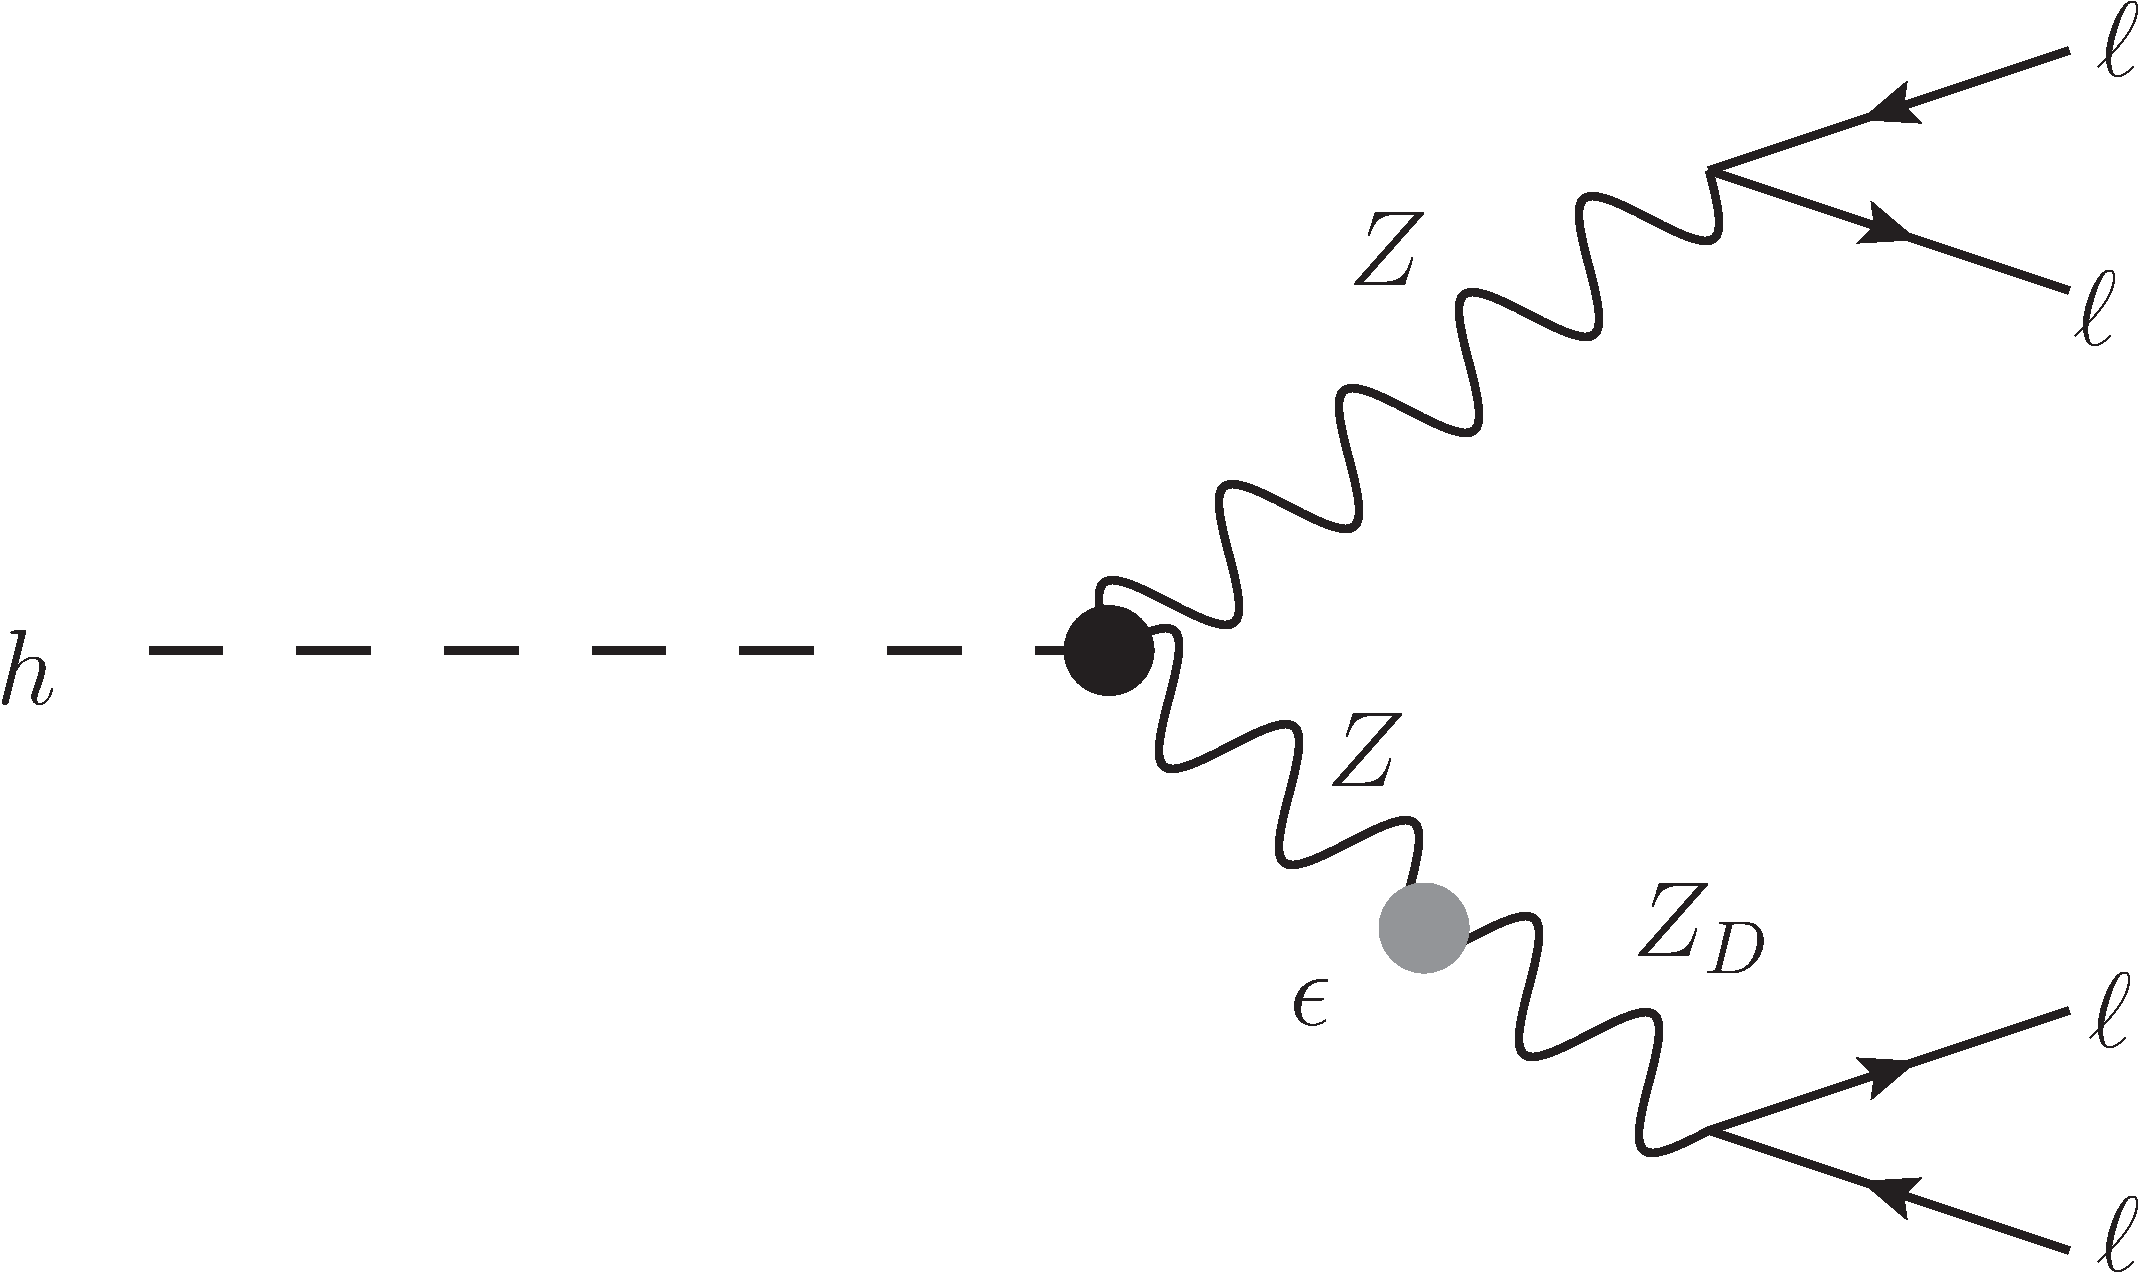
\includegraphics[width=0.4 \textwidth]{section9/plots/feynmandiagram_hzzd}
& \hspace{4mm} &
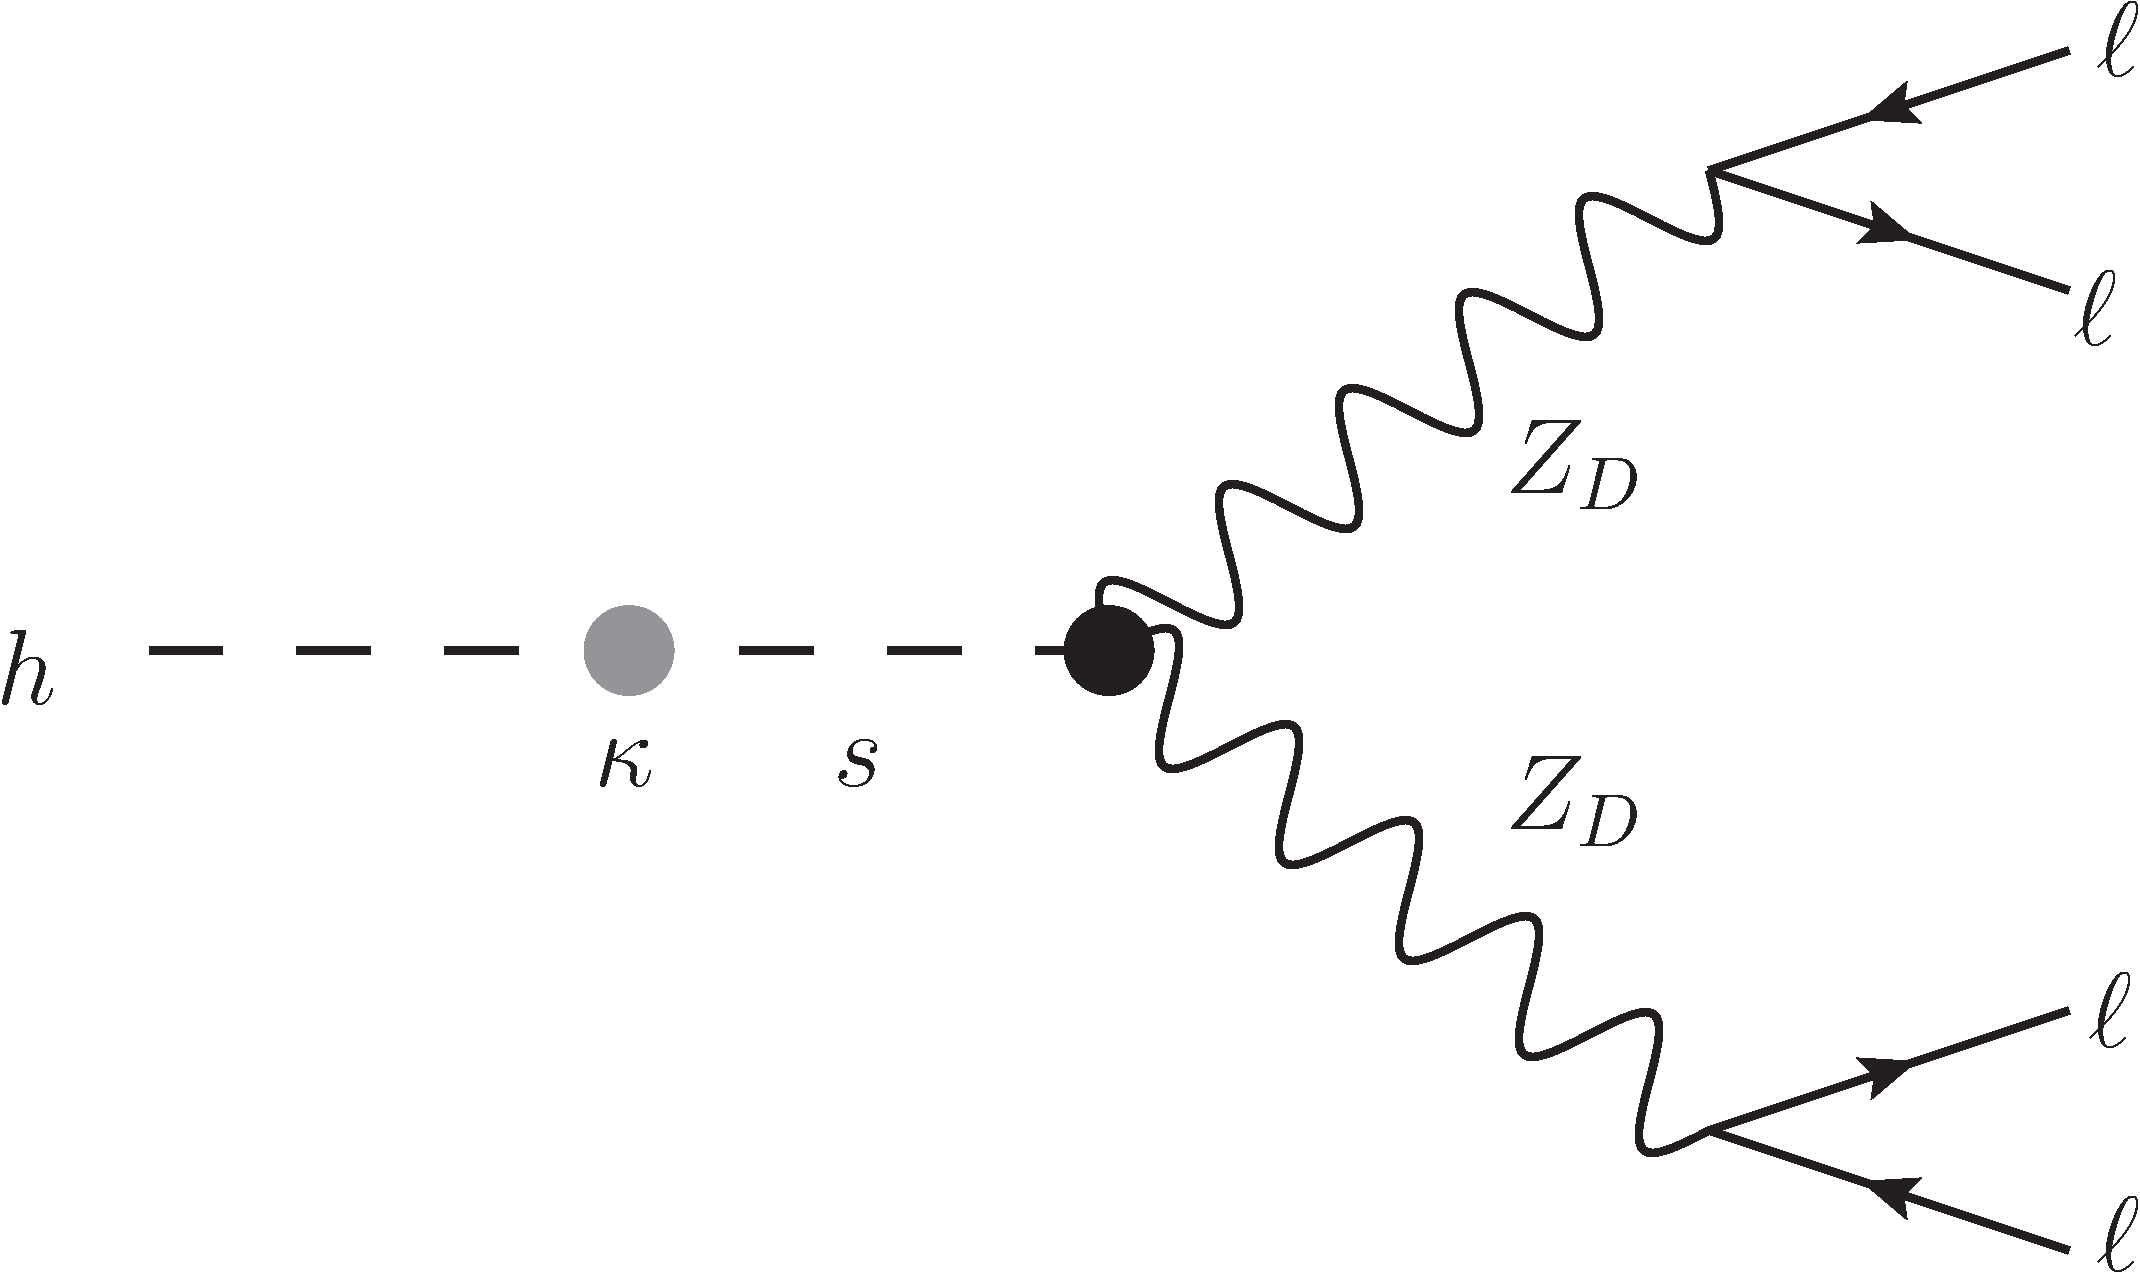
\includegraphics[width=0.4\textwidth]{section9/plots/feynmandiagram_hzdzd}
\end{tabular}
\end{center}
\caption{ Exotic Higgs decays to four leptons induced by intermediate
  dark photons in the higgsed dark $U(1)$ model. \emph{Left:} $h\to Z_D
  Z^{(*)} \to 4\ell$ via the photon portal. \emph{Right:} $h \to Z_D Z_D
  \to 4\ell$ via the Higgs portal. }
\label{f.ZDfeynman}
\end{figure}
%%%%%%%%%%%%%%%%%%%%%%%%%%%%%%%%%%%%%%%%%%%%


% explain  main ways to probe this model: exotic higgs decays via kinetic mixing (ZZD), DY, exotic higgs decays via higgs mixing


This simplified model gives rise to two kinds of exotic Higgs decays, shown in Fig.~\ref{f.ZDfeynman}. The first is decay through the \emph{photon portal}: kinetic mixing between $Z$ and $Z_D$ allows for $h\to Z_D Z^{(\star)}$, with $\mathrm{Br} \propto \epsilon^2$. The second is decay through the \emph{higgs portal}: mixing between $h$ and $s$ allows for $h \to Z_D Z_D$ with $\mathrm{Br} \propto \kappa^2$. We discuss these decays in more detail below, but we note that dark photon models can give rise to other signals as well. 
%
Kinetic mixing gives rise to DY-like production of dark photons and a resulting dilepton resonance via $p p \to Z_D \to \ell^+ \ell^-$. This probes the same coupling as $h \to Z_D Z^{(\star)}$ and, as we discuss below, tends to have slightly greater sensitivity. 
%
If the dark higgs and dark photon masses are in a suitable range, the so-called ``platinum channel'' becomes available~\cite{Izaguirre:2018atq}, where $h \to 2s \to 4 Z_D \to 8 \ell$ with $\mathrm{Br} \propto \kappa^2$. We do not discuss this in detail here, but this final state is extremely conspicuous, and if this channel is available, the corresponding low-background search could have significantly greater sensitivity to exotic Higgs decay branching ratio  than the example of $h \to Z_D Z_D$ we study here. 
%
The mass spectrum could also allow for exotic $Z$-decays~\cite{Blinov:2017dtk} via an intermediate dark higgs, $Z \to Z_D s \to Z_D Z_D Z_D$. 
%
Finally, all these signatures could be dressed up or augmented by signatures of a non-minimal hidden sector, where the dark photon/higgs could decay into invisible stable particles and/or LLPs (see e.g. \cite{Alexander:2016aln, Curtin:2018mvb}).
% \DC{cite, comment... Yuhsin NN, etc?}
%
The space of possible signatures is clearly very rich. Even so, the simple benchmark decays we examine here give a feeling for the physics reach of the HL- and HE-LHC in probing these kinds of theories. 

\bigskip

\paragraph{Decays through the photon portal}
% ZZD / DY


\begin{figure}
\begin{tabular}{m{0.5 \textwidth} m{0.4\textwidth}}
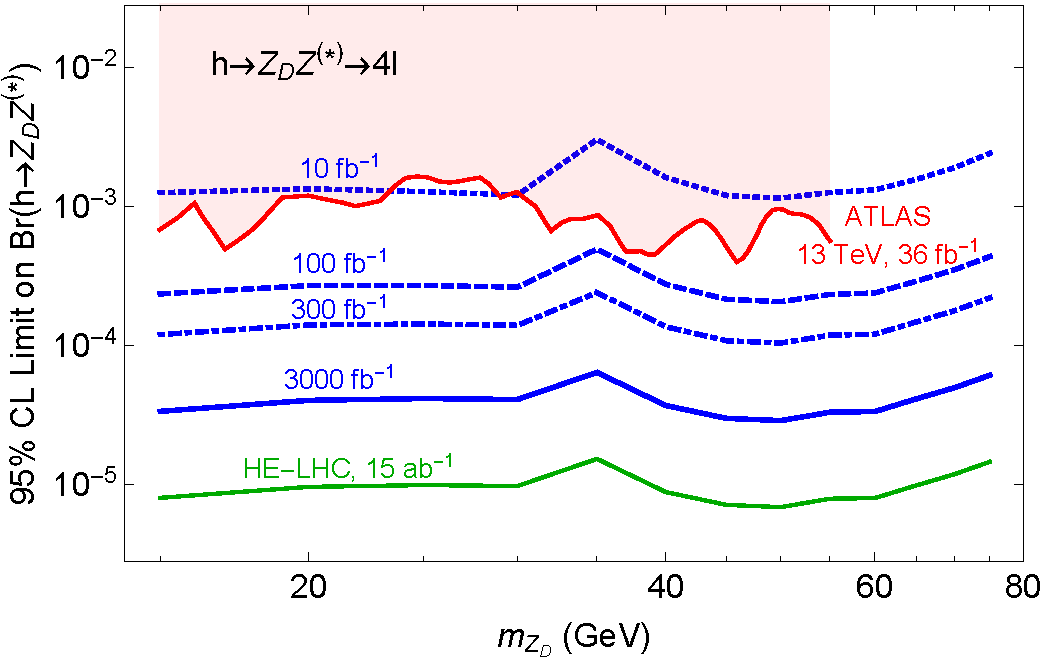
\includegraphics[width=0.5\textwidth]{section9/plots/zzdbrplot}
&
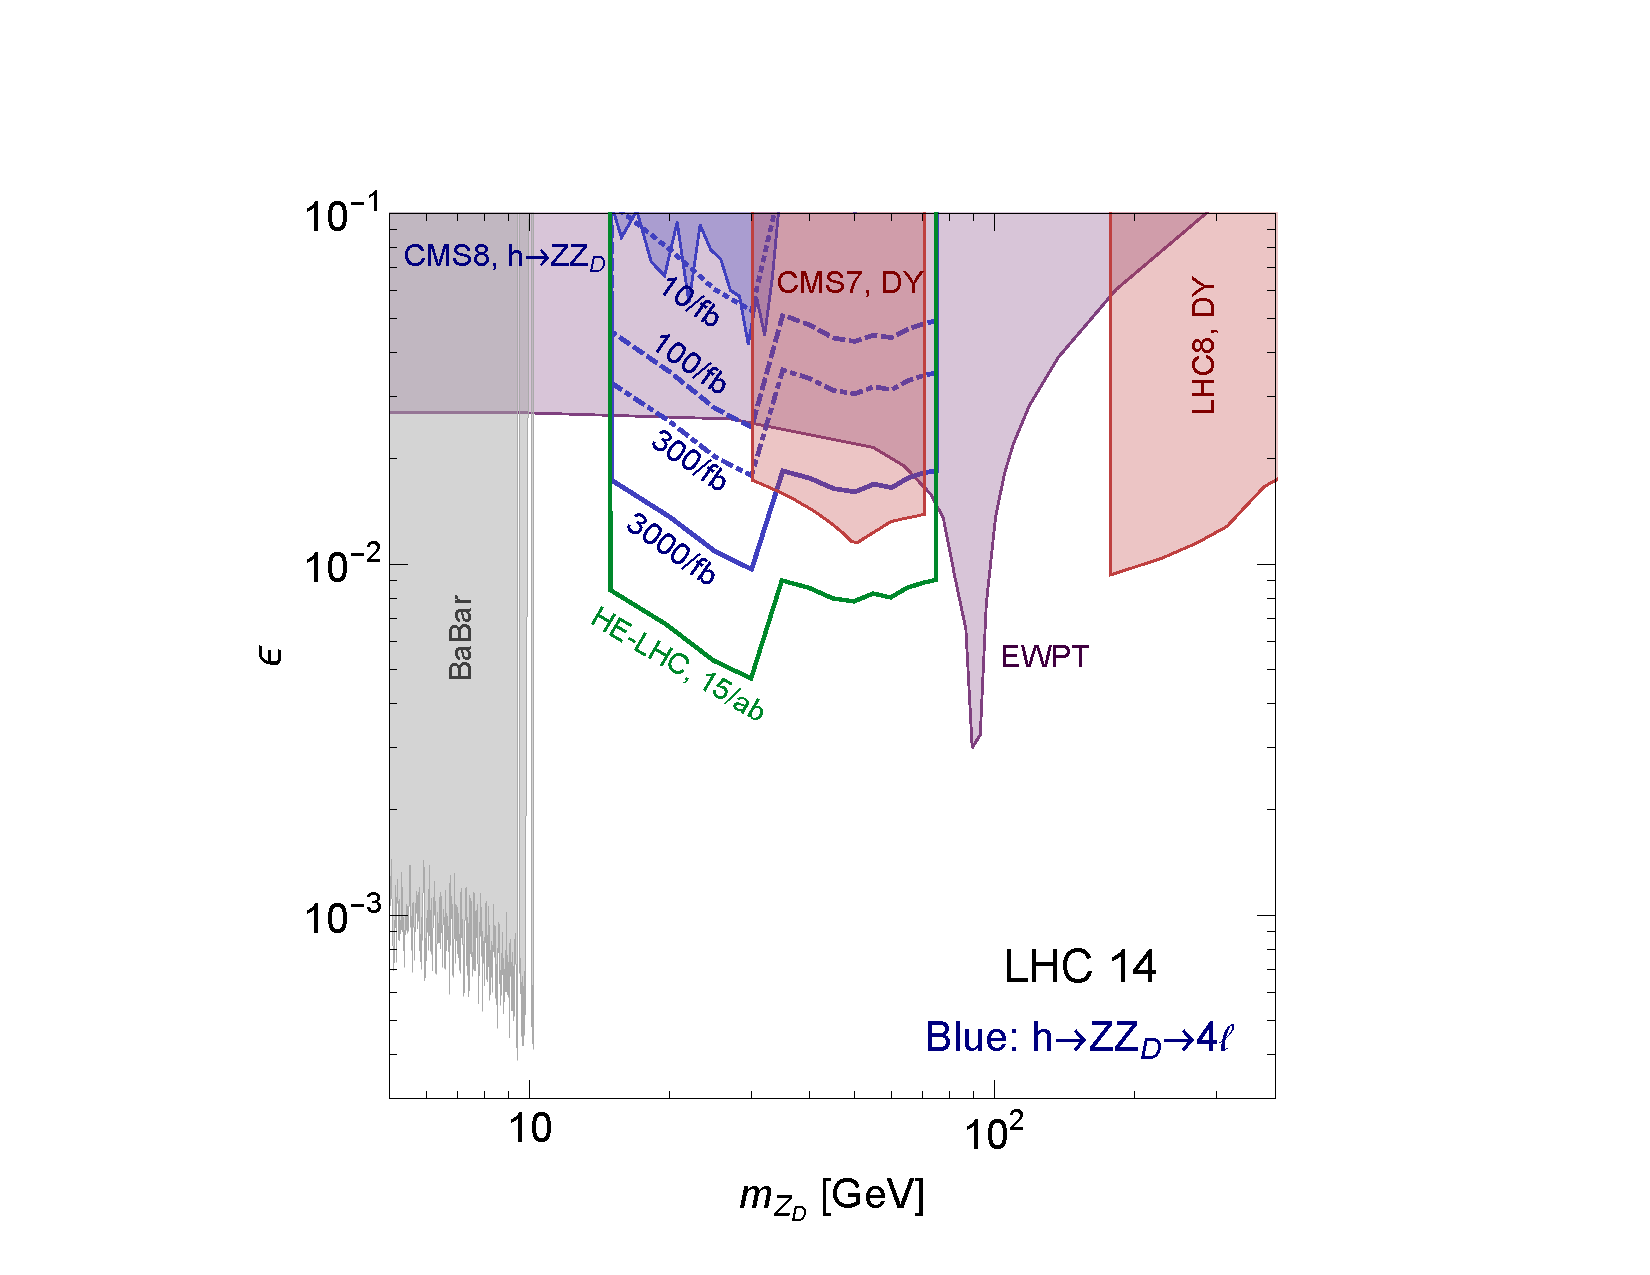
\includegraphics[width=0.4\textwidth]{section9/plots/new_zzdplot_epsilon}
\end{tabular}
\caption{
Sensitivity of the (HL-)LHC and HE-LHC to  $h \to Z_D Z^{\star} \to 4 \ell$ decays, as a function of dark photon mass and exotic Higgs decay branching ratio (left) or dark photon kinetic mixing parameter $\epsilon$ (right). Figures taken from~\cite{Curtin:2014cca} with the addition of the HE-LHC projection and the recent experimental limit from~\cite{Aaboud:2018fvk}.
%
 Blue contours, taken from~\cite{Curtin:2014cca}, correspond to the reach of $14 \tev$ $pp$ collisions with the HL-LHC sensitivity indicated by a solid blue curve. The green contour corresponds to the HE-LHC at $\sqrt{s} = 27 \tev$ with 15 $\mathrm{ab}^{-1}$ of luminosity, and is derived by rescaling the 14 TeV projections for 27 TeV signal and background cross sections, see text for details. The red shaded region on the right shows the exclusions from the recent ATLAS search at 13 TeV with 36 fb$^{-1}$~\cite{Aaboud:2018fvk}.
}
\label{f.darkphotonZZD}
\end{figure}



Kinetic mixing of the dark photon can allow the Higgs to undergo the decay $h \to Z_D Z^{\star}$ shown in Fig.~\ref{f.ZDfeynman} (a). A search for the four-lepton ($e$ or $\mu$) final state has the best sensitivity, making use of the known invariant mass of the higgs and the assumed mass peak in the invariant mass of one of the lepton pairs. The HL-LHC sensitivity of such a search was estimated in~\cite{Curtin:2014cca} and is shown in Fig.~\ref{f.darkphotonZZD}. 
%
Exotic higgs branching ratios of few$\times 10^{-5}$ can be probed. 
%
The projected limits of~\cite{Curtin:2014cca} can be approximately rescaled for the HE-LHC if the increase in signal and background cross section (as a function of $m_{Z_D}$) are known. 
%
The signal increases simply in accordance with the greater higgs production cross section at 27 TeV compared to 14 TeV.
%
The increase in background generally depends on $m_{Z_D}$, since this determines the applied invariant mass cuts. To estimate this background increase, we simulate the two main backgrounds to the four-lepton final state, di-$Z/\gamma$ and $h \to Z Z^*$ production, in Madgraph at parton level for 14 and 27 TeV and apply the analysis cuts of~\cite{Curtin:2014cca}.
%
The resulting increase in background rate is quite $m_{Z_D}$-indepedent, since background is dominated by SM higgs decays. We therefore adopt a uniform factor of 4.2  for the HE-LHC branching ratio sensitivity increase compared to the HL-LHC, and the resulting projection is shown as the green contour in Fig.~\ref{f.darkphotonZZD}.
%
We also show the recent exclusions obtained by the ATLAS 13 TeV search for this decay with 36 fb$^{-1}$~\cite{Aaboud:2018fvk}, which agrees roughly with our projections for LHC reach. 


The reach in exotic Higgs branching ratio is impressive, below the $10^{-5}$ level at the HE-LHC.
This allows exotic Higgs decay sensitivities on the kinetic mixing parameter better than $10^{-2}$, approaching the best sensitivity of current electroweak precision constraints, see Fig.~\ref{f.darkphotonZZD} (right). 
%
Even so, exotic Higgs decays are not the most probe of $\epsilon$ in this model. Instead, simple DY production of $Z_D$ and search for the resulting dilepton resonance on top of the $Z^*$ background still has the greatest reach in $\epsilon$, see Fig.~\ref{f.darkphotonDY} from~\cite{Curtin:2014cca}. For this figure, HE-LHC constraints are also derived from the 14 TeV projections by rescaling the signal and background cross sections as a function of $m_{\ell \ell} \approx m_{Z_D}$. Here, the HE-LHC could reach sensitivities better than $\epsilon \sim 10^{-3}$. 

It is important to point out that while exotic Higgs decays may not be the most sensitive probe of kinetic mixing in this scenario, they nevertheless serve an important function in diagnosing the dark sector. Discovery of a resonance in the DY spectrum could indicate a conventionally coupled $Z'$ or a kinetically mixed dark photon. However, a  discovery of the  corresponding exotic Higgs decay would strongly suggest the latter scenario. 


\begin{figure}
\begin{center}
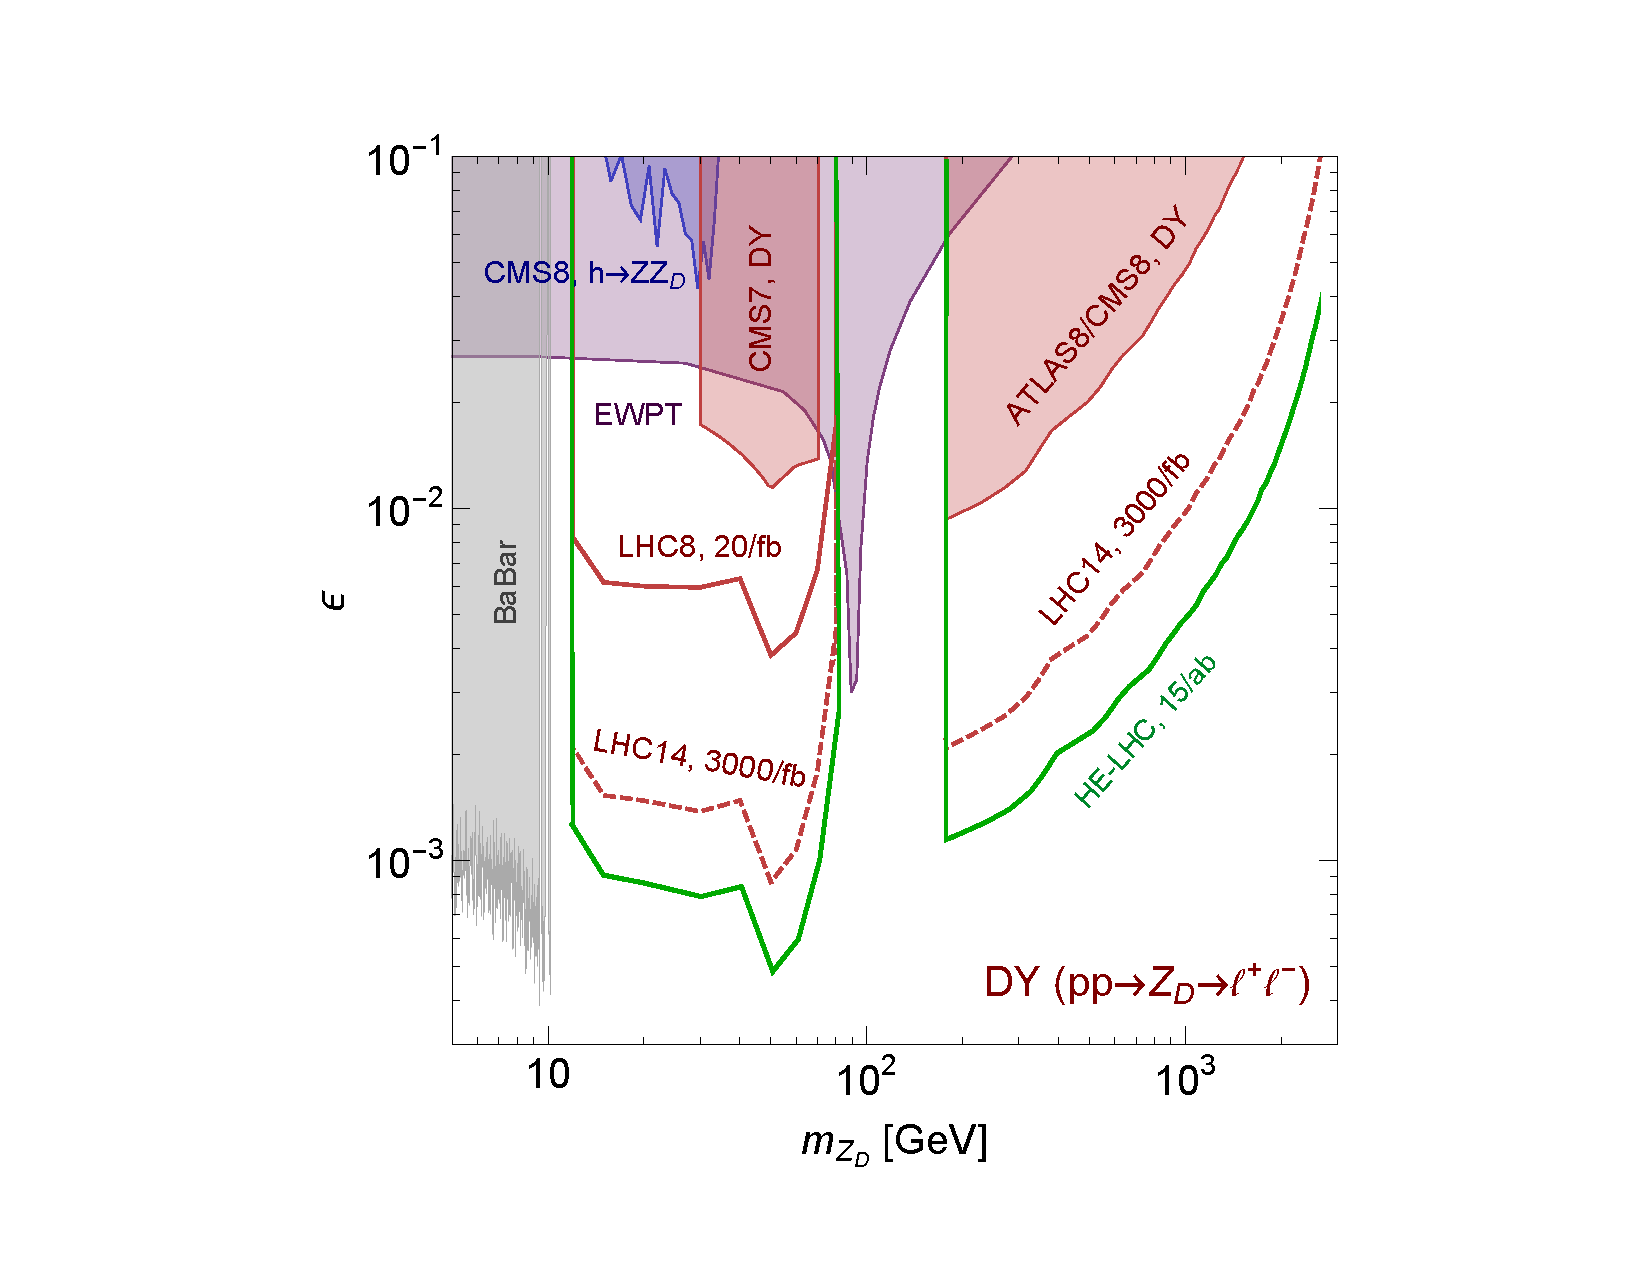
\includegraphics[width=0.5\textwidth]{section9/plots/new_DYplot_epsilon}
\end{center}
\caption{
Sensitivity of the (HL-)LHC and HE-LHC to DY production of $Z_D$ and decay to two leptons,  as a function of dark photon mass and kinetic mixing parameter $\epsilon$. Figure taken from~\cite{Curtin:2014cca}, indicating the sensitivity of searches at 14 TeV (red contours) with the HL-LHC sensitivity indicated by the red dashed curve. The added green contour corresponds to the HE-LHC at $\sqrt{s} = 27 \tev$ with 15 $\mathrm{ab}^{-1}$ of luminosity, and is derived by rescaling the 14 TeV projections for 27 TeV signal and background cross sections, see text for details. 
}
\label{f.darkphotonDY}
\end{figure}


\bigskip

\paragraph{Decays through the Higgs portal}

If the dark photon obtains its mass from a dark Higgs mechanism, one would generally expect there to be nonzero mixing with the SM higgs. This can lead to exotic Higgs decays to dark photons, as shown in Fig.~\ref{f.ZDfeynman} (b). 


The signal is independent of $\epsilon$ as long as it is large enough for $Z_D$ to decay promptly. 
%
Again, the four-lepton final state is the best search target, and the requirement of two diliepton invariant masses coincident at $m_{Z_D}$ and $m_{4 \ell} \approx m_h$ is a very stringent signal requirement that greatly suppresses backgrounds. 
%
The sensitivity projections for the HL-LHC are shown in Fig.~\ref{f.darkphotonZDZDprompt}, with exotic Higgs as small as $\times 10^{-6}$ being observable. 
%
We rescale these limits for the HE-LHC in an identical manner to the previous two analyses, with the resulting projection shown as the green contour. The low background of the search means sensitivity increases almost proportional to the increased signal rate at higher energy and luminosity, allowing branching ratios below $10^{-7}$ to be probed, corresponding to tiny higgs portal couplings of $\kappa \sim 10^{-5}$. 

% ZDZD prompt

\begin{figure}
\begin{tabular}{m{0.45 \textwidth} m{0.45\textwidth}}
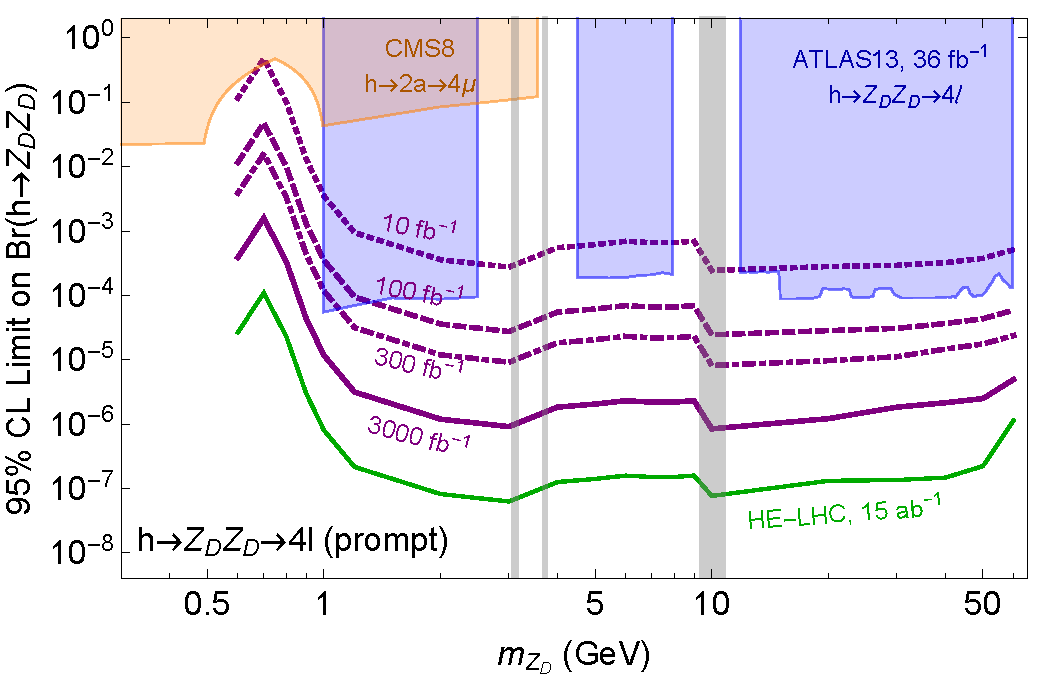
\includegraphics[width=0.45\textwidth]{section9/plots/FORPAPER_HiggsMixingLimitsBrHZdZd_14_27_TeV}
&
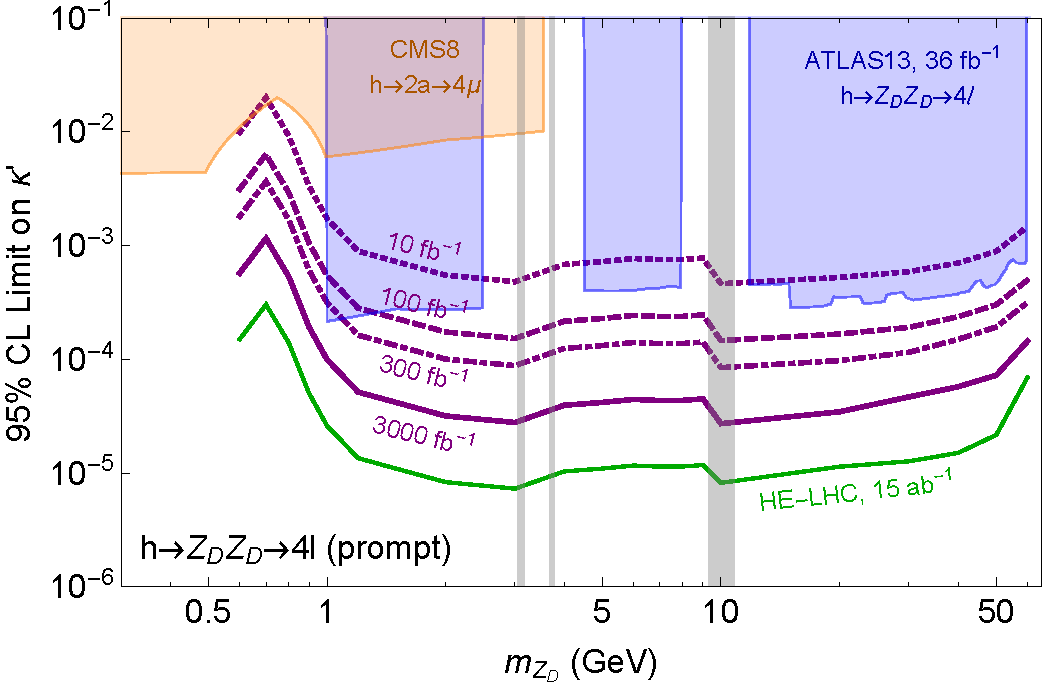
\includegraphics[width=0.45\textwidth]{section9/plots/FORPAPER_HiggsMixingLimitskappaprime_14_27_TeV}
\end{tabular}
\caption{
Sensitivity of the (HL-)LHC and HE-LHC to  $h \to Z_D Z_D$ decays, where each $Z_D$ decays to $ee$ or $\mu \mu$ promptly. Limits are shown as a function of dark photon mass and exotic Higgs decay branching ratio (left) or higgs mixing parameter $\kappa$ (right). 
%
Figures taken from~\cite{Curtin:2014cca} with the addition of the HE-LHC projection and the recent experimental limit from~\cite{Aaboud:2018fvk}.
%
 Purple contours, taken from~\cite{Curtin:2014cca}, correspond to the reach of $14 \tev$ $pp$ collisions with the HL-LHC sensitivity indicated by a solid purple curve. The green contour corresponds to the HE-LHC at $\sqrt{s} = 27 \tev$ with 15 $\mathrm{ab}^{-1}$ of luminosity, and is derived by rescaling the 14 TeV projections for 27 TeV signal and background cross sections, see text for details. The blue shaded regions sho the exclusions from the recent ATLAS search at 13 TeV with 36 fb$^{-1}$~\cite{Aaboud:2018fvk}.
}
\label{f.darkphotonZDZDprompt}
\end{figure}


% ZDZD displaced

For very small $\epsilon$, the $Z_D$ decay is displaced, becoming a long-lived particle (LLP). In this case, exotic Higgs decays play a uniquely important role in probing the dark sector, since the photon portal could be far too small to serve as a production mechanism, while the Higgs portal could be wide open. 
%
This was analyzed in~\cite{Curtin:2014cca,Curtin:2018mvb}. 



 
 
























%%%%%%%%%%%%%%%%%%%%%%%%%%%%%%%%%%%%%%%

%%%%%%%%%%%%%%%%%%%%%%%%%%%%%%%%%%%%%%%
%\bibliography{newbibfile}
%\bibliographystyle{JHEP}

%%%%%%%%%%%%%%%%%%%%%%%%%%%%%%%%%%%%%%%


%\end{document}




